\section{Security of Global Navigation Satellite Systems GNSS}

\paragraph{Overview}
Orbiting satellites transmit their location and a precise timestamp.
Receivers collect these navigation messages and their arrival time and use \textbf{triangulation} to calculate their own position.
Satellites are positioned such that at least four are always in sight on any point on Earth.

Three segments: users, satellites, ground control.%
\footnote{There are of course issues with special and general relativity that mess with the time.}

\paragraph{Signalling}
Each satellite modulates the navigation message with a spreading code (coarse acquisition C/A for civilians (public), precision P/Y for military (secret)).
The spread signal is then modulated onto a carrier.
\\
Individual satellites use individual spreading codes to allow distinction.
\\
GPS sends on two carrier frequencies at the same time, L1 (1575.42 MHz = 10.23 MHz $\times$ 154) and L2 (1227.60 MHz = 10.23 MHz $\times$ 120).%
\footnote{This only applies to military. The civilian C/A is only transmitted on L1.}
Apart from jamming resistance and redundancy, this also allows to calculate the ionospheric delay error.
\\
Due to atmospheric attenuation, down on Earth the GPS signal is well below the thermal noise.

\paragraph{Navigation message}
Each message consists of 25 frames.
Each takes 30 sec to transmit, so the total time is 12.5 min.
\\
Each frame contains: satellite clock + health data, 2x ephemeris (orbit details), other data + almanac (orbital + clock details).

\paragraph{Time of Arrival TOA}
Travel time of the signal from the satellite to the receiver.
Used to calculate the distance and thus eventually the receiver position.
Found by sliding the spreading code over the received message until a correlation peak.

\paragraph{Spoofing attacks}
Messages are unauthenticated (for practical reasons, else they would become too long).
\\
By sending stronger signals, overshadowing the legitimate ones, an attacker can modify the \textit{navigation message contents} (transmission time, satellite location) or their \textit{time of arrival} (retransmitting captured signals with a temporal shift), resulting in a wrong location being calculated.
\\
This is an issue in civilian GPS (messages can be generated and delayed) as well as in military GPS (messages can only be delayed since they are encrypted).
Unfortunately, commercial GPS signal generators are becoming increasingly cheap.


\subsection{Spoofing Detection and Mitigation}

\paragraph{Types of countermeasures}
\begin{itemize}
	\item \textbf{Infrastructure/protocol:} e.g. cryptographic authentication of navigation messages
	\item \textbf{Receivers:}
	Use physical-layer characteristics of the signal to validate the signal as well as the calculated position/velocity/time.
	E.g. direction of arrival, carrier phase, signal strength, etc.
\end{itemize}

\paragraph{Angle of Arrival AoA}
Use multiple antennas (e.g. on both ends of a ship) to calculate the angle of arrival through the phase difference and the known distance between the antennas (see beam steering, \autoref{fig:beam-steering}).
In a spoofed scenario, the angles would all be very similar.
Restricts the locations from which the attacker can successfully spoof.

\underline{Problems:}
Attacker can use drones to spoof signal from more realistic angle.
Reflection of legitimate signal of buildings (thus reaching the receiver at a shallower angle) could be wrongly classified as spoofing.
Computationally expensive phase measurement.
Hardware modification.

\paragraph{Monitor Signal Characteristic Changes}
Over time, monitor signal properties such as AGC (Automatic Gain Control), noise level, number of satellites, spatial diversity (AoA) or the autocorrelation peak.
Abrupt changes in any of these indicate presence of spoofing.

\paragraph{Seamless takeover attack}
The attacker starts transmitting a copy of a legitimate GPS signal in sync with the original one, but at low power, having no influence on the receiver.
Then the attacker slowly starts increasing the power, until the receiver prefers the attacker signal.
Now the attacker can change the GPS signal, and the receiver will keep following. 

\begin{figure}
	\centering
	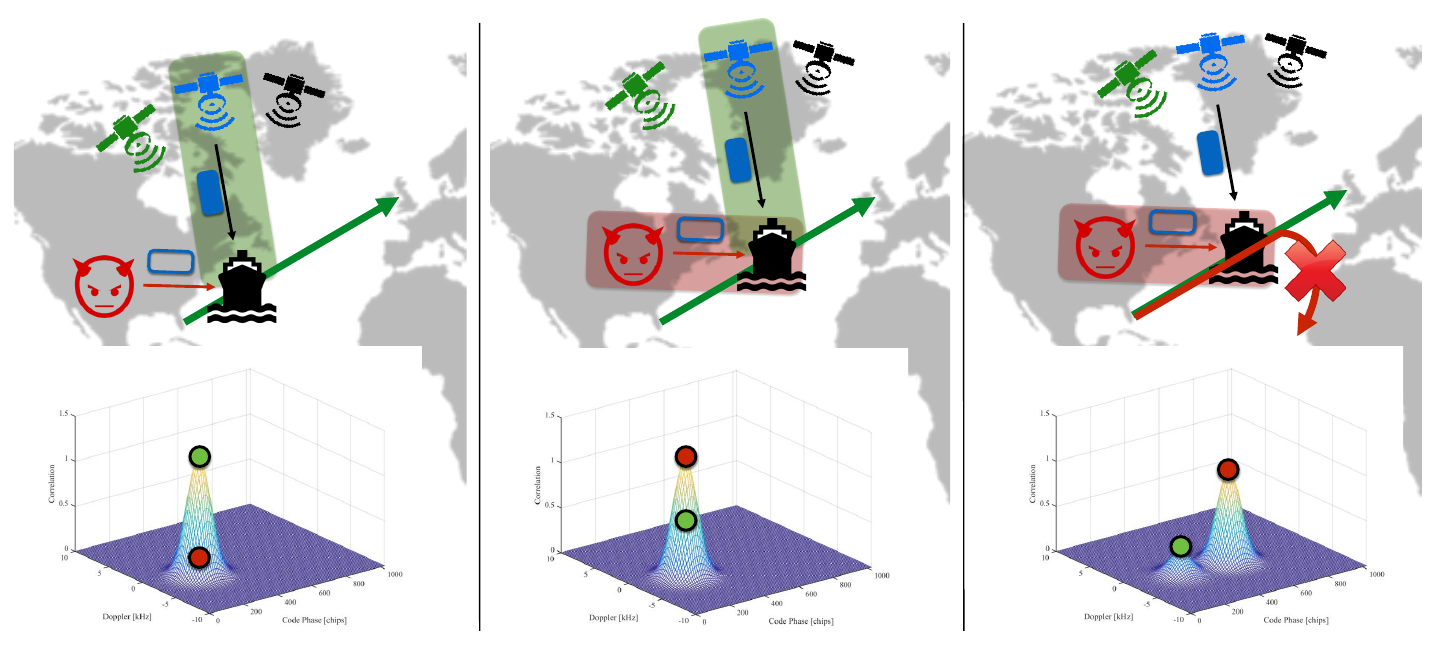
\includegraphics[scale=0.4]{images/4-seamless-takeover.png}
	\caption{Seamless takeover attack}
	\label{fig:seamless-takeover}
\end{figure}

\paragraph{SPoofing REsistance GPS rEceiver SPREE}
Leverage peak tracking (of \underline{all} signal peaks) to detect seamless takeover attacks.
Navigation message inspection detects content spoofing.

\paragraph{Cryptographic approach (Kuhn)}
\begin{enumerate}
	\item At time $t$: satellite uses secret spreading code.
	Receiver uses a broadband receiver to capture the entire band.
	\item At time $t+dt$: Satellite disclosed code, signing the disclosure with its secret key.
	Receiver verifies signature, de-spreads the signal.
\end{enumerate}

\underline{Advantages:}
Prevents fake signal generation and individual signal delay.

\underline{Disadvantages:}
Requires pre-shared public satellite keys.
Does NOT prevent full-band delay.
Slightly inefficient (longer latency until signal lock).
Replay attacks (?).

